\documentclass{beamer}
\usepackage{graphicx}
\usepackage{listings}
\usepackage{hyperref}
\usepackage{xcolor}
\usepackage{fontawesome5}
\usepackage{tcolorbox}
% Removing enumitem package as it conflicts with beamer's enumeration
% \usepackage{enumitem}
\usepackage{tikz}

% Define colors
\definecolor{myblue}{RGB}{41,128,185}
\definecolor{mygreen}{RGB}{46,204,113}
\definecolor{myred}{RGB}{231,76,60}
\definecolor{mypurple}{RGB}{155,89,182}
\definecolor{myorange}{RGB}{243,156,18}

% Set theme
\usetheme{Madrid}
\usecolortheme{beaver}
\setbeamertemplate{navigation symbols}{}
\setbeamertemplate{blocks}[rounded][shadow=true]

% Title page info
\title{Navigating Programming Education in AI Age}
\subtitle{From Syntax Details to System Design}
\author{Workshop Facilitator}
\date{\today}
\institute{Faculty Workshop}

\begin{document}

% Title slide
\begin{frame}
    \titlepage
\end{frame}

% Overview slide
\begin{frame}{Workshop Overview}
    \begin{itemize}
        \item \textbf{Duration:} 1 hour
        \item \textbf{Target Audience:} Instructors of programming-oriented university courses
        \item \textbf{Format:} Interactive, hands-on
    \end{itemize}
    
    \begin{tcolorbox}[colback=myblue!10,colframe=myblue,title=Workshop Objectives]
        \begin{itemize}
            \item Explore evolving role of AI in programming education
            \item Experience multiple levels of AI programming assistance
            \item Design classroom activities that integrate AI support
            \item Shift focus from coding mechanics to design thinking 
        \end{itemize}
    \end{tcolorbox}
\end{frame}

% Agenda slide
\begin{frame}{Agenda}
    \begin{enumerate}
        \item \textbf{Introduction} [10 min]
            \begin{itemize}
                \item AI as new abstraction level
                \item Paradigm shift in programming 
            \end{itemize}
        
        \item \textbf{AI Programming Assistance Levels} [15 min]
            \begin{itemize}
                \item \faRocket~Level 1: Auxiliary Code Generation
                \item \faSearch~Level 2: Code Review \& Improvement
                \item \faBrain~Level 3: Copilot Integration
                \item \faPuzzlePiece~Level 4: Agent Mode for Complex Projects
            \end{itemize}
        
        \item \textbf{Hands-on Design Activity} [20 min]
        
        \item \textbf{Show \& Tell / Discussion} [15 min]
    \end{enumerate}
\end{frame}

% Introduction: Increasing Abstraction
\begin{frame}{Increasing Abstraction Levels in Programming}
    \begin{center}
        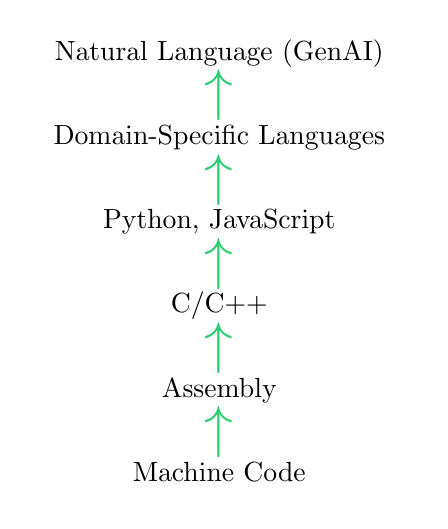
\begin{tikzpicture}
            \node[align=center] at (0,0) {
                \begin{tabular}{c}
                    Natural Language (GenAI) \\
                    \textcolor{mygreen}{\huge $\uparrow$} \\
                    Domain-Specific Languages \\
                    \textcolor{mygreen}{\huge $\uparrow$} \\
                    Python, JavaScript \\
                    \textcolor{mygreen}{\huge $\uparrow$} \\
                    C/C++ \\
                    \textcolor{mygreen}{\huge $\uparrow$} \\
                    Assembly \\
                    \textcolor{mygreen}{\huge $\uparrow$} \\
                    Machine Code
                \end{tabular}
            };
        \end{tikzpicture}
    \end{center}

    \begin{itemize}
        \item Higher abstractions = more complex systems with less code
        \item Focus shifts to system design rather than implementation details
        \item Initial concerns: performance, loss of control
        \item Natural language: newest abstraction level with GenAI
    \end{itemize}
\end{frame}

% Paradigm Shift
\begin{frame}{Paradigm Shift in Programming}
    \begin{columns}
        \column{0.5\textwidth}
        \textbf{GenAI as Peer Programmer}
        \begin{itemize}
            \item Generates scripts with natural language
            \item Reviews \& improves existing code
            \item Helps with code patterns \& completion
            \item Develops multi-file projects
        \end{itemize}
        
        \column{0.5\textwidth}
        \textbf{Changing Programmer Role}
        \begin{itemize}
            \item From syntax to design \& intent
            \item From contributor to team lead
            \item Enables larger-scale projects
            \item Still needs understanding of entire stack
        \end{itemize}
    \end{columns}
    
    \begin{alertblock}{Aircraft Autopilot Analogy}
        \begin{itemize}
            \item Autopilot handles low-level tasks, but pilot maintains control
            \item Pilot still needs system understanding to identify \& address issues
        \end{itemize}
    \end{alertblock}
\end{frame}

% Limitations
\begin{frame}{Limitations of GenAI}
    \begin{block}{Not a Replacement for Human Programmers}
        \begin{itemize}
            \item Can generate code, but driven by human creativity \& problem-solving
            \item Limited to abstractions from training data
            \item Cannot build novel, high-impact projects independently
            \item Helps build projects faster with less effort on implementation details
        \end{itemize}
    \end{block}
    
    \begin{center}
        \large \textbf{Key Question:} \\
        How do we guide students to become technology leaders while ensuring they understand underlying details?
    \end{center}
\end{frame}

% Level Overview
\begin{frame}{AI Programming Assistance Levels}
    \begin{tcolorbox}[colback=myblue!5,colframe=myblue,title=Increasing Complexity \& Integration]
        \begin{enumerate}
            \item \textbf{\textcolor{myblue}{\faRocket~Level 1:} Auxiliary Code Generation}\\
            One-shot generation of scripts beyond course focus
            
            \item \textbf{\textcolor{myred}{\faSearch~Level 2:} Code Review \& Improvement}\\
            Analyze, debug, enhance existing code with AI feedback
            
            \item \textbf{\textcolor{mygreen}{\faBrain~Level 3:} Copilot Integration}\\
            Contextual code completion with intent-driven prompts
            
            \item \textbf{\textcolor{mypurple}{\faPuzzlePiece~Level 4:} Agent Mode for Complex Projects}\\
            Agentic AI systems for multi-file, complex codebases
        \end{enumerate}
    \end{tcolorbox}
\end{frame}

% Level 1: Auxiliary Code Generation
\begin{frame}{Level 1: Auxiliary Code Generation}
    \begin{block}{Pedagogical Framing}
        \begin{itemize}
            \item In-depth courses need focused attention on core topic
            \item Not enough time to cover out-of-domain details
            \item AI generates auxiliary code: data loaders, visualizations, diagnostics
        \end{itemize}
    \end{block}
    
    \begin{alertblock}{Example: Real-time Analysis in Embedded Systems}
        Students develop Linux kernel modules for PWM signals, but need analysis code:
        \begin{itemize}
            \item AI generates data visualization to analyze signal quality
            \item Students focus on core learning while gaining insights from analysis
            \item Enables experiential learning in larger context
        \end{itemize}
    \end{alertblock}
\end{frame}

% Level 1: Example
\begin{frame}{Level 1: Example Visualization Output}
    \begin{figure}
        \centering
        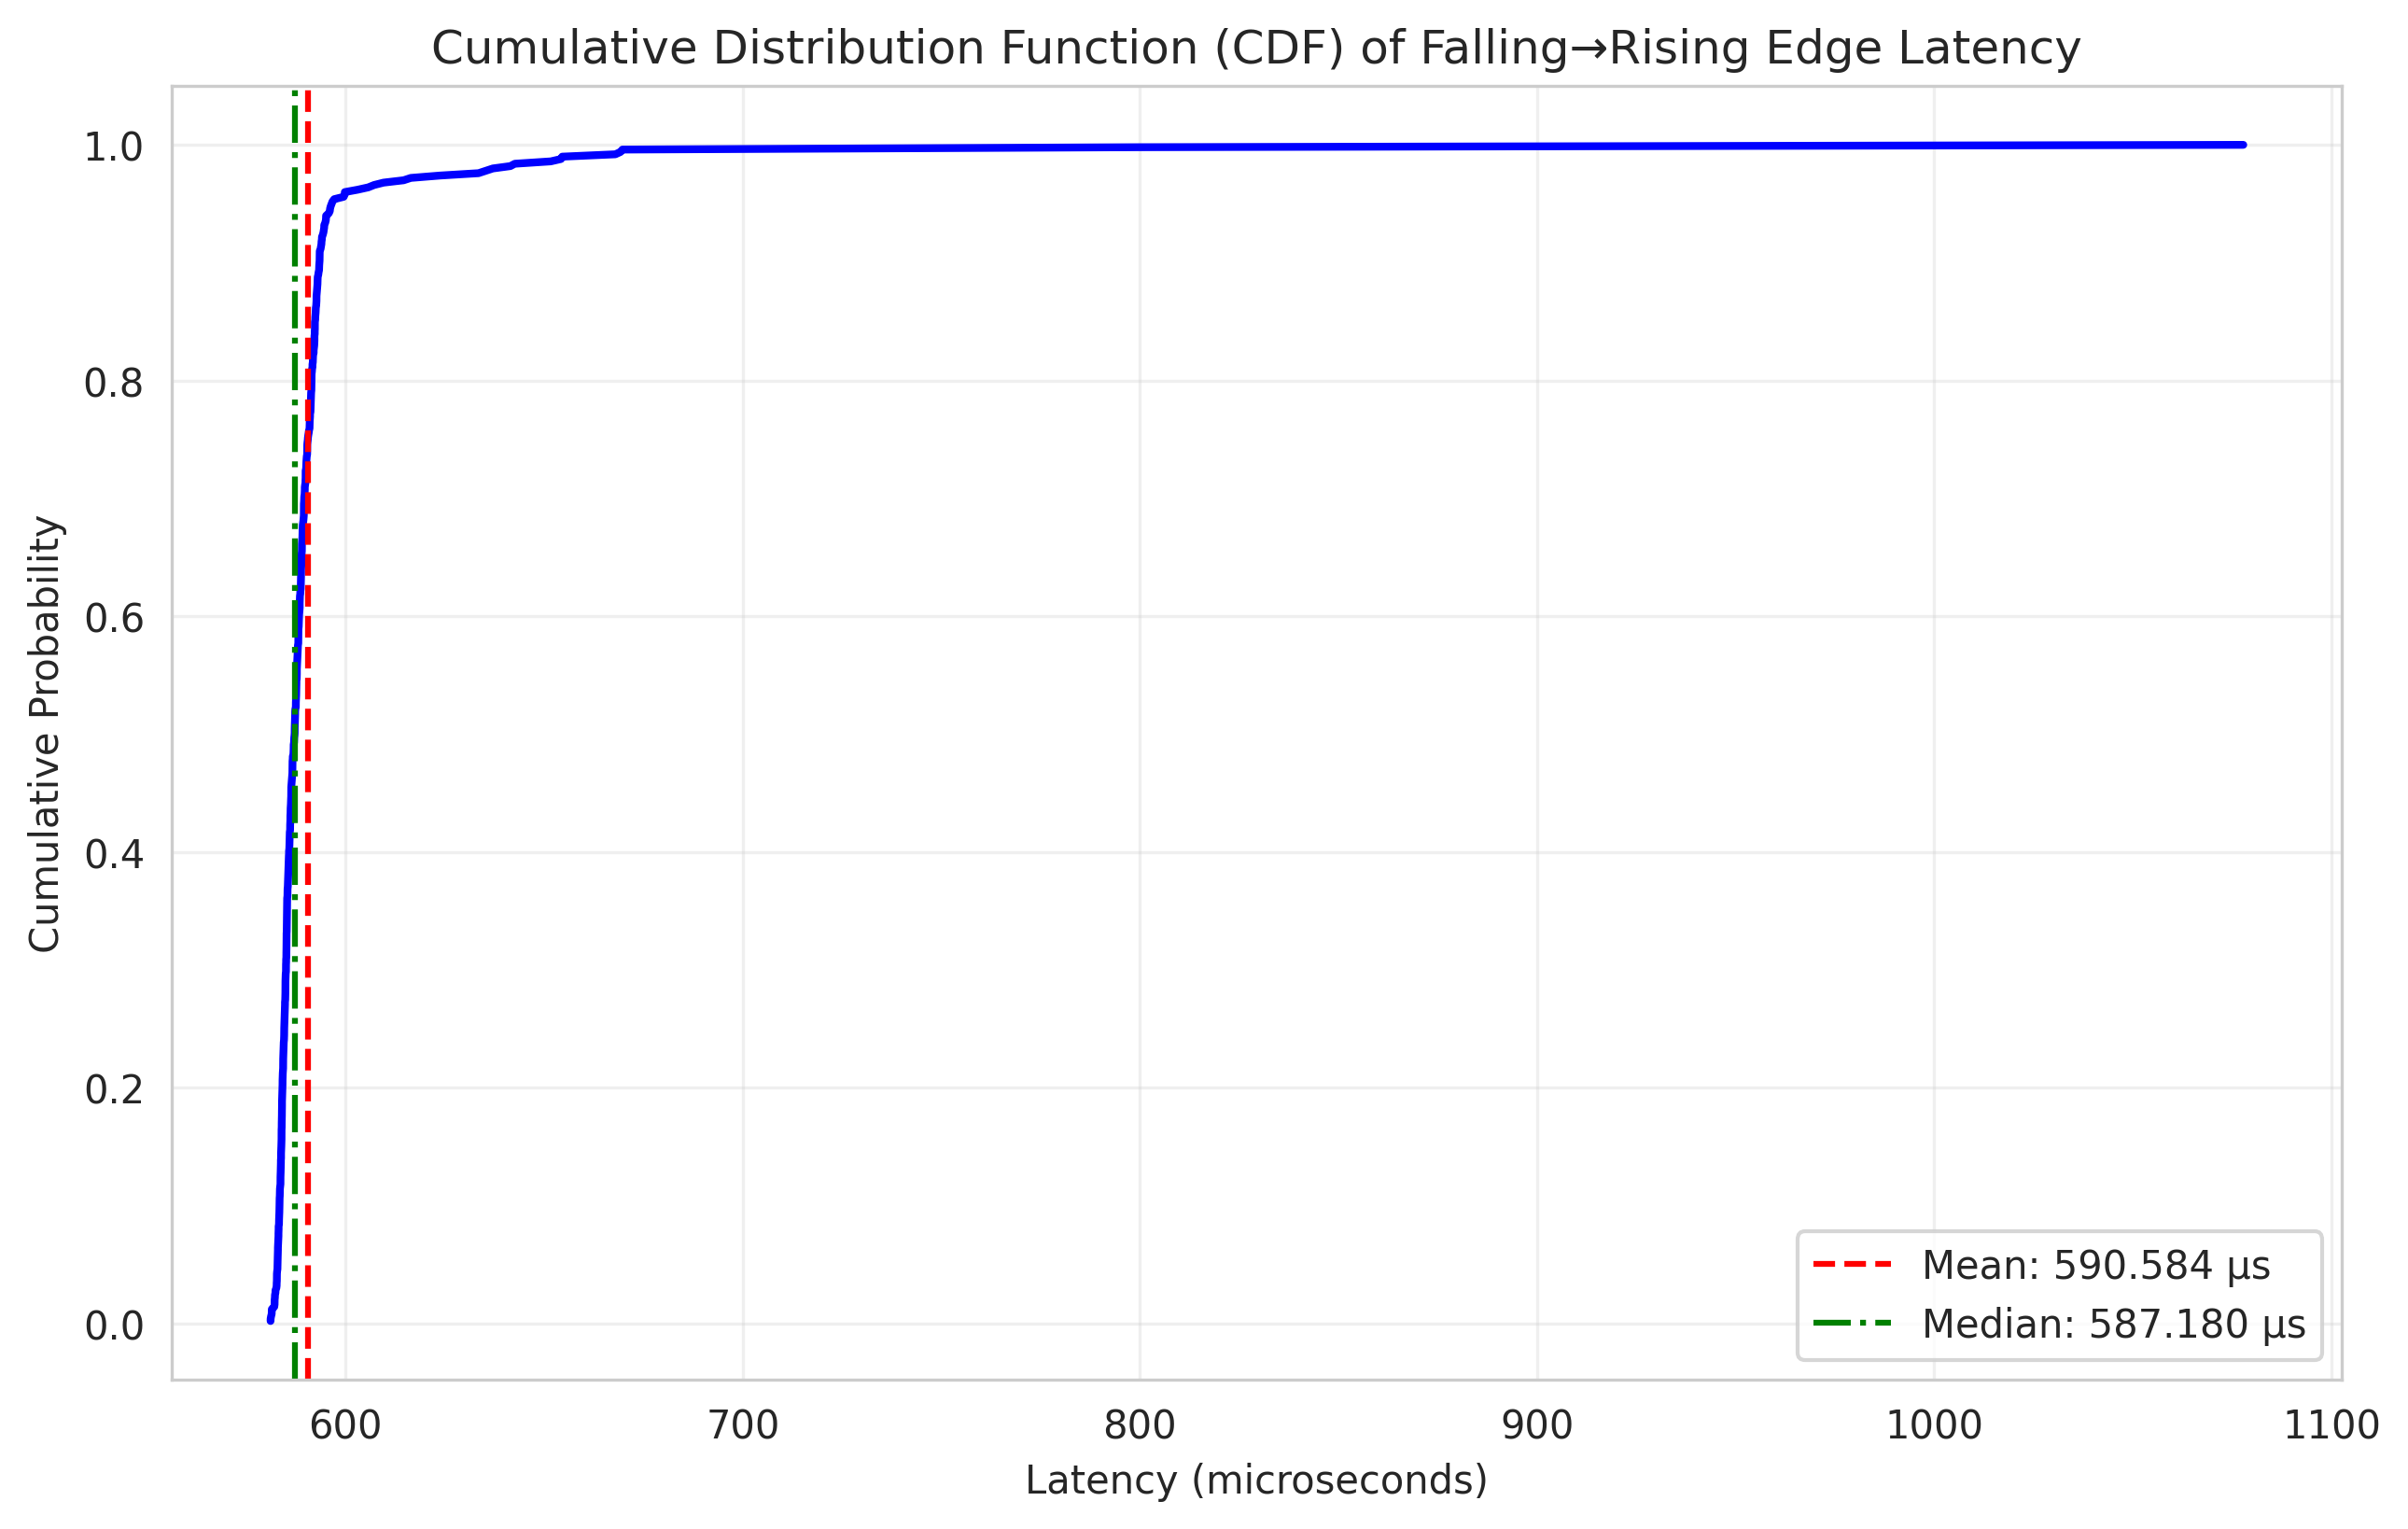
\includegraphics[width=0.8\textwidth]{/home/schirner/work/ai-prog-workshop/1-script/pwm_sleep_edges_loaded_latency_cdf.png}
        \caption{AI-generated visualization of falling-to-rising edge latency}
    \end{figure}
\end{frame}

% Level 1: Implementation Methods
\begin{frame}{Level 1: Implementation Methods Comparison}
    \begin{columns}
        \column{0.33\textwidth}
        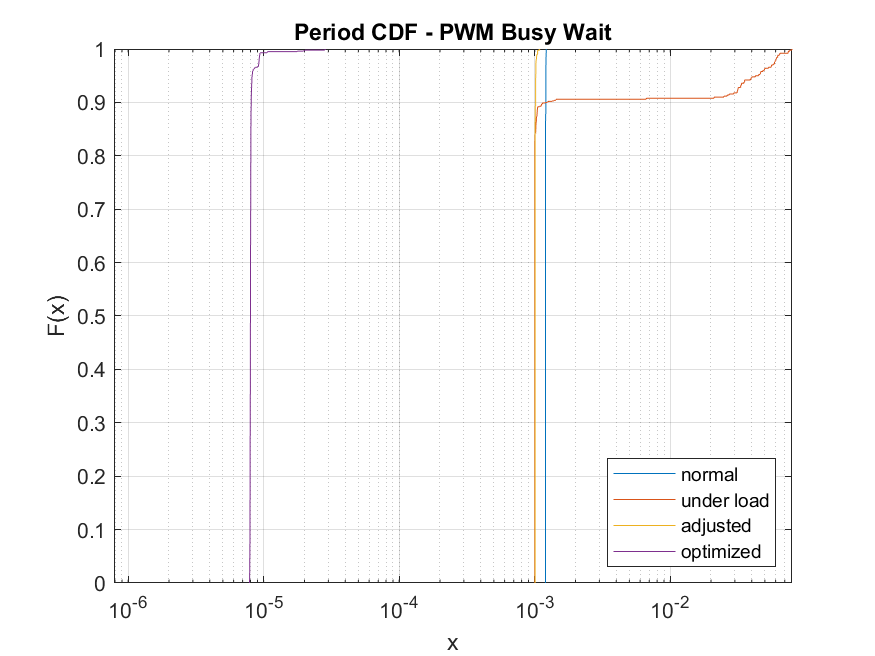
\includegraphics[width=\textwidth]{/home/schirner/work/ai-prog-workshop/1-script/period_busy.png}
        \centering (a) Busy Loop
        
        \column{0.33\textwidth}
        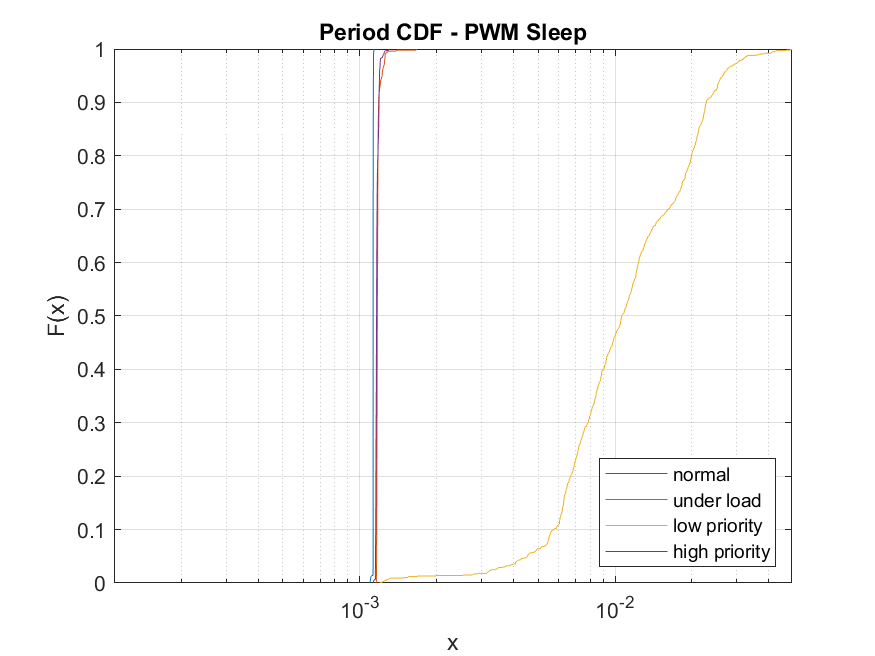
\includegraphics[width=\textwidth]{/home/schirner/work/ai-prog-workshop/1-script/period_sleep.png}
        \centering (b) OS Sleep
        
        \column{0.33\textwidth}
        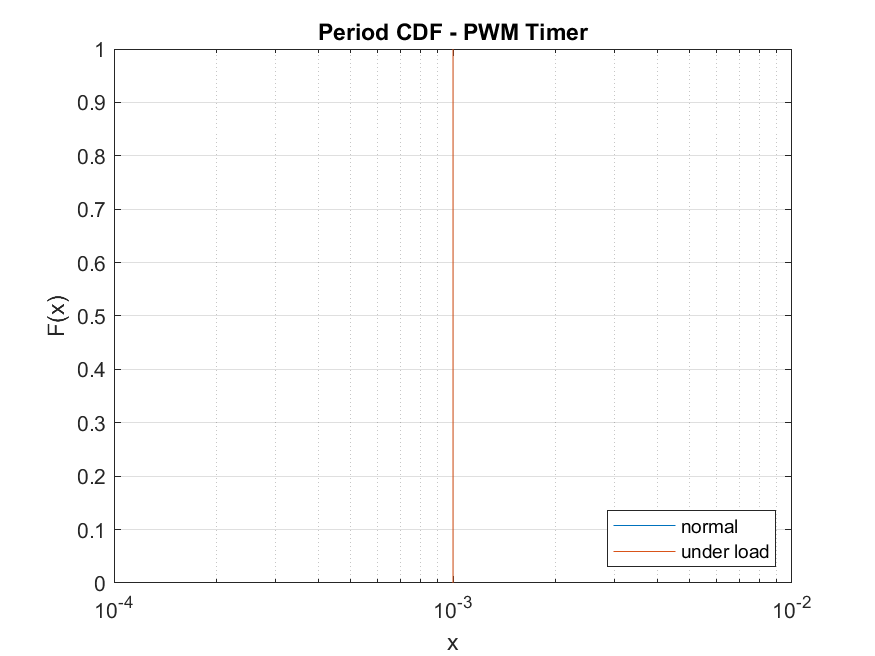
\includegraphics[width=\textwidth]{/home/schirner/work/ai-prog-workshop/1-script/period_timer.png}
        \centering (c) Hardware Timer
    \end{columns}
    
    \begin{itemize}
        \item Generated visualization code allows students to compare implementation methods
        \item Focus on what impacts real-time quality without burden of visualization code
    \end{itemize}
\end{frame}

% Level 1: Prompting
\begin{frame}{Level 1: AI Prompting Examples}
    \begin{tcolorbox}[colback=mygreen!5,colframe=mygreen,title=Sample Prompt]
        "I need a Python script to analyze timing data from digital signals. I have a CSV file with the following columns:
        1. Sample Time (in seconds)
        2. Edge type (0 for RISING, 1 for FALLING)
        3. Duration since last edge of same type (seconds)
        4. Duration since last edge of opposite type (seconds)
        
        Please write a script that:
        1. Reads the CSV file
        2. Extracts the latency between falling and rising edges 
        3. Calculates and plots the cumulative probability distribution (CDF)
        4. Adds appropriate labels, title, and grid
        5. Displays basic statistics (mean, median, min, max, std)
        6. Saves the plot as a PNG file"
    \end{tcolorbox}
    
    \begin{itemize}
        \item Clear, specific task description 
        \item Specifies exact requirements and expected outputs
        \item Focuses on what, not how (implementation details left to AI)
    \end{itemize}
\end{frame}

% Level 2: Code Review
\begin{frame}{Level 2: AI as Code Review \& Improvement Tool}
    \begin{block}{Pedagogical Framing}
        \begin{itemize}
            \item AI as a coach, not solving problems directly
            \item Scaffold problem-solving process
            \item Students analyze code first, then get AI hints
            \item Promotes:
                \begin{itemize}
                    \item Deeper understanding of algorithms
                    \item Collaborative learning through AI discussion
                    \item Debugging as discovery
                \end{itemize}
        \end{itemize}
    \end{block}
\end{frame}

% Level 2: Example
\begin{frame}[fragile]{Level 2: Merge Sort Example}
    \begin{tcolorbox}[colback=myred!5,colframe=myred,title=Faulty Merge Sort Code]
        \begin{lstlisting}[language=Python, basicstyle=\tiny\ttfamily]
def merge_sort(arr):
    if len(arr) <= 1:
        return arr

    mid = len(arr) // 2
    left = merge_sort(arr[:mid])
    right = merge_sort(arr[mid]) 

    return merge(left, right)

def merge(left, right):
    sorted_list = []
    i = j = 0
    while i < len(left) or j < len(right):
        
        if i < len(left) and (j >= len(right) or left[i] < right[j]):
            sorted_list.append(left[i])
            i += 1
        else:
            sorted_list.append(right[j])
            j += 1

    return sorted_list
        \end{lstlisting}
    \end{tcolorbox}
    
    \begin{itemize}
        \item Students analyze first, identify possible bugs
        \item Then use AI to confirm understanding or get hints
    \end{itemize}
\end{frame}

% Level 2: AI Feedback
\begin{frame}{Level 2: AI Code Review Feedback}
    \begin{tcolorbox}[colback=myred!5,colframe=myred,title=AI-Identified Issues]
        \begin{enumerate}
            \item \textbf{Incorrect Slice in Recursive Call}
                \begin{itemize}
                    \item \texttt{right = merge\_sort(arr[mid])} should be \texttt{arr[mid:]}
                \end{itemize}
                
            \item \textbf{Unsafe Loop Condition}
                \begin{itemize}
                    \item \texttt{while i < len(left) or j < len(right)} should use \texttt{and}
                \end{itemize}
                
            \item \textbf{Missing Appending of Remaining Elements}
                \begin{itemize}
                    \item Need to add unprocessed elements after the loop
                \end{itemize}
        \end{enumerate}
    \end{tcolorbox}
    
    \begin{itemize}
        \item AI provides specific feedback and explanations
        \item Students learn to identify subtle bugs
        \item Promotes critical evaluation of AI's reasoning
    \end{itemize}
\end{frame}

% Level 3: Copilot Integration
\begin{frame}{Level 3: Copilot Integration for Code Completion}
    \begin{block}{Pedagogical Framing}
        \begin{itemize}
            \item Copilot as design collaborator, not just solution engine
            \item Translate high-level intent into functional code
            \item Shifts focus from syntax to design thinking
            \item Students make critical decisions about suggestions
        \end{itemize}
    \end{block}
    
    \begin{figure}
        \centering
        \includegraphics[width=0.5\textwidth]{/home/schirner/work/ai-prog-workshop/3-assist/copilot_intro.gif}
        \caption{Copilot suggesting code based on intent}
    \end{figure}
\end{frame}

% Level 3: Example Output
\begin{frame}{Level 3: Example - Clustering Visualization}
    \begin{figure}
        \centering
        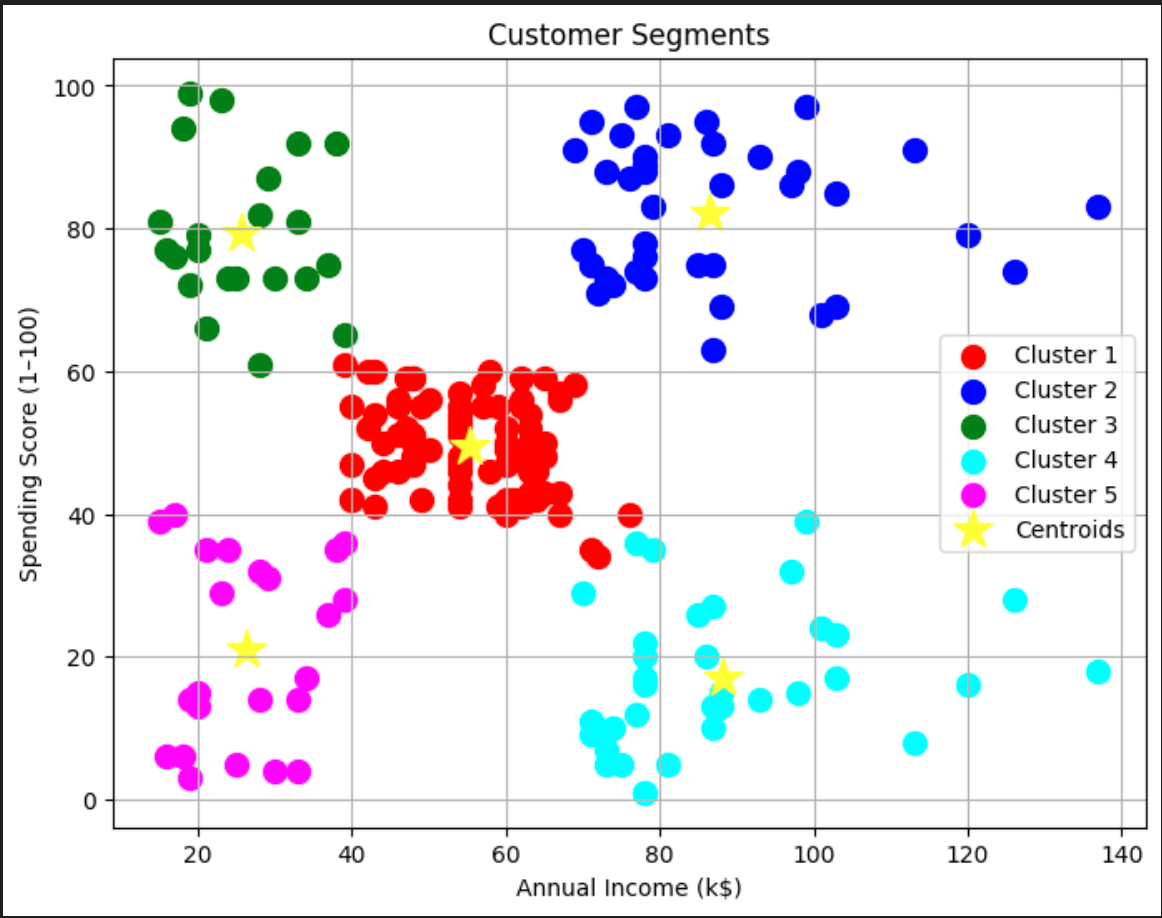
\includegraphics[width=0.7\textwidth]{/home/schirner/work/ai-prog-workshop/3-assist/Cluster.jpeg}
        \caption{Cluster visualization result from Copilot-assisted code}
    \end{figure}
    
    \begin{itemize}
        \item Students specify intent ("cluster these points and visualize them")
        \item Copilot generates appropriate functions and visualizations
        \item Students focus on interpretation and design decisions
    \end{itemize}
\end{frame}

% Level 4: Agent Mode
\begin{frame}{Level 4: Agent Mode for Complex Projects}
    \begin{block}{Vibe Coding Overview}
        \begin{itemize}
            \item Rapid prototyping and collaborative iteration with AI
            \item Prioritizes UX and system flow over low-level details
            \item Enables quick project scaffolding and experimentation
            \item Growing adoption in startups (25\% of YC cohort use mostly AI-generated code)
        \end{itemize}
    \end{block}
    
    \begin{alertblock}{Pedagogical Framing}
        \begin{itemize}
            \item Experiential learning through hands-on projects
            \item Time constraints (4-6 weeks) limit scope
            \item Agent Mode enables more ambitious projects
            \item Students focus on architecture and design
            \item Challenge: understanding large volumes of generated code
        \end{itemize}
    \end{alertblock}
\end{frame}

% Level 4: Example
\begin{frame}{Level 4: Example - Group Organization Tool}
    \begin{tcolorbox}[colback=mypurple!5,colframe=mypurple,title=Project Requirements]
        Web application that:
        \begin{itemize}
            \item Allows participants to log in with just their name
            \item Lets users select from predefined interest areas
            \item Enables an admin to finalize group formation
            \item Automatically pairs participants based on shared interests
            \item Displays team assignments to all participants
            \item Provides a simple team chat functionality
        \end{itemize}
    \end{tcolorbox}
    
    \begin{itemize}
        \item Complex, multi-file project with front-end, back-end, and real-time communication
        \item Would normally require weeks to implement
        \item Agent Mode generates functional application from high-level description
    \end{itemize}
\end{frame}

% Level 4: Project Structure
\begin{frame}[fragile]{Level 4: Project Structure Generated by Agent}
    \begin{lstlisting}[basicstyle=\tiny\ttfamily]
group-organizer/
├── client/                 # Frontend React application
│   ├── public/
│   └── src/
│       ├── components/     # UI components
│       │   ├── Login.js
│       │   ├── InterestSelection.js
│       │   ├── AdminPanel.js
│       │   ├── TeamDisplay.js
│       │   └── Chat.js
│       ├── contexts/       # State management
│       ├── App.js
│       └── index.js
├── server/                 # Backend Express application
│   ├── models/             # Data models
│   ├── routes/             # API endpoints
│   ├── socket/             # WebSocket handlers
│   └── index.js
└── package.json
    \end{lstlisting}
    
    \begin{itemize}
        \item Agent Mode designs complete project architecture
        \item Implements components across front-end and back-end
        \item JSON-based storage for persistence
        \item WebSocket for real-time updates
    \end{itemize}
\end{frame}

% Classroom Activities Design
\begin{frame}{Designing AI-Integrated Classroom Activities}
    \begin{columns}
        \column{0.5\textwidth}
        \textbf{Level 1: Auxiliary Code}
        \begin{itemize}
            \item Identify tasks beyond course scope
            \item Craft detailed prompts for script generation
            \item Focus on understanding outputs over implementation
        \end{itemize}
        
        \textbf{Level 2: Code Review}
        \begin{itemize}
            \item Select appropriate buggy algorithms
            \item Structure AI interaction for hints not answers
            \item Require reflection on AI feedback
        \end{itemize}
        
        \column{0.5\textwidth}
        \textbf{Level 3: Copilot Integration}
        \begin{itemize}
            \item Start with partially written code
            \item Focus on clear intent expression
            \item Critical evaluation of suggestions
        \end{itemize}
        
        \textbf{Level 4: Agent Projects}
        \begin{itemize}
            \item Define complex, multi-component projects
            \item Create detailed system specifications
            \item Assess system design understanding
        \end{itemize}
    \end{columns}
\end{frame}

% Hands-on Activity
\begin{frame}{Hands-on Activity}
    \begin{tcolorbox}[colback=myorange!5,colframe=myorange,title=Design an AI-Integrated Classroom Activity]
        \begin{enumerate}
            \item Select an AI assistance level that fits your course
            \item Identify a specific programming concept or challenge
            \item Design a structured activity that uses AI appropriately
            \item Consider prompts, student workflow, and assessment
        \end{enumerate}
    \end{tcolorbox}
    
    \begin{itemize}
        \item Work individually or in small groups (10-15 minutes)
        \item Document your activity design
        \item Prepare to share with the larger group
    \end{itemize}
\end{frame}

% Discussion
\begin{frame}{Discussion \& Reflection}
    \begin{block}{Key Questions}
        \begin{itemize}
            \item How does AI change what we emphasize in programming education?
            \item What new skills become more important for students?
            \item How do we balance AI assistance with fundamental understanding?
            \item What assessment methods work in an AI-assisted context?
        \end{itemize}
    \end{block}
    
    \begin{alertblock}{Moving Forward}
        \begin{itemize}
            \item Course redesign considerations
            \item Developing AI literacy alongside programming skills
            \item Creating appropriate guardrails vs. open exploration
            \item Preparing students for AI-augmented professional environments
        \end{itemize}
    \end{alertblock}
\end{frame}

% Resources
\begin{frame}{Resources \& Next Steps}
    \begin{tcolorbox}[colback=myblue!5,colframe=myblue,title=AI Tools for Programming Education]
        \begin{itemize}
            \item GitHub Copilot (\url{https://github.com/features/copilot})
            \item GitHub Copilot Agent Mode (\url{https://github.blog/news-insights/product-news/github-copilot-agent-mode-activated/})
            \item Claude (\url{https://claude.ai}) for script generation
            \item Y Combinator: The Rise of Vibe Coding (\url{https://www.ycombinator.com/blog/the-rise-of-vibe-coding/})
        \end{itemize}
    \end{tcolorbox}
    
    \begin{alertblock}{Next Steps}
        \begin{itemize}
            \item Review workshop materials at your own pace
            \item Experiment with integrating one AI tool into your course
            \item Start small with a low-stakes activity
            \item Share experiences with colleagues
        \end{itemize}
    \end{alertblock}
\end{frame}

% Thank You
\begin{frame}{Thank You!}
    \begin{center}
        \huge{Questions \& Discussion}
        
        \vspace{1cm}
        
        \large{Workshop Materials:} \\
        \texttt{github.com/yourrepository/ai-prog-workshop}
    \end{center}
\end{frame}

\end{document}
